\subsection{Designing}
This phase of the project is the ground of all development.
Implementation results are meant to come up into one playable game, which is later used for testing.
\subsubsection{Unity Game Engine}
The testing area now consists of three primary things: a spherical object representing a 360 view, the ground floor of any type, and a simulated tank environment.
Using some basic knowledge from the Gaming Industry unit, the tank is now capable of moving by applying basic mechanics.\\
A sphere around the tank will simulate a real-world reality.
Top the tank contains another object, a sit for a player.
This location will be a placement for VR Glasses, where the Player controls the tank.
It represented as a VR camera view, which was provided by SteamVR prefab, with a place for controller events.
This environment is meant to simulate a real Mixed Reality experience using a headset and controllers.\\[1pc]
%The rest, regarding calculating distance, is simple math using cameras property. By detecting an object and placing hitting box around, it marks as a potential target. Shooting from a barrel will require some time to implement. \\
The process of integrating new features on top of the previous work went much smoother with updated versions of the components. 
If in the previous Unity was an entirely new environment for an Engineer, now, with the support of the supervisor and general practice with a Gaming Industry unit, project quality got improved.
The goal of the project remains the same, to present whatever discovery achieved during the investigation.\\[1pc]
In the future, the tester will have the possibility to manipulate with objects.
With interaction using controllers, the gamer must have all the means to move a tank inside the environment and, therefore, see how Unity will simulate precisely the same behaviour with the real tank.
Any manipulation will be recorded and sent back to the Engine for a 360-degree view.
FFmpeg Library and Machine Learning will be able to capture the stream and modify it with proper masking, marking enemy tanks.
With assistance from unity markers and barrel controllers, the player is meant to feel himself in a simulation of immersive experience - tank commander target practice, which will be detected by Unity and scored for every successful hit.
This kind of simulation is what project aims, and so far, it achieved significant progress.
\subsubsection{$360\circ$ camera}	
In the early stages of the project, camera reconstruction appeared as a square box around the player, as shown in subfigure~\ref{fig:oldLook}. 
Now, using an updated Movie texture plugin and modified stream, the entire surrounding is reconstructed over a hemisphere. 
A new look is represented on subfigure~\ref{fig:newLook}.
This section will cover the process in detail.\\
A square box did not provide a clear image over the surrounding area, and the way the video appeared on squares always changed itself with every run. 
That is why an example prefabs contained a spherical example too.
However, the tricky part was to reverse texture from the outside view, into inside.\\    
This operation is achieved by reversing a sphere shader.
It was a matter of trial and error to get a proper look, but a new Shader, which came from Unity documentation, has the following look in Appendix~\ref{apx:shader}. \\[1pc]
Another trial is cutting a sphere in half. 
The stream from a camera contained half the sphere output, which was directed within unity to cover the entire sphere.
Half of the image had to disappear, which caused a view loss.
One of the performed trials was to create an actual hemisphere object using a Blender 3D model, which was a success.
However, Applying a texture on top of that caused a similar loss.
Except for the wasted time, the idea brought no results.
\begin{figure}[H]
	\centering
	\begin{subfigure}[b]{0.4\textwidth}
		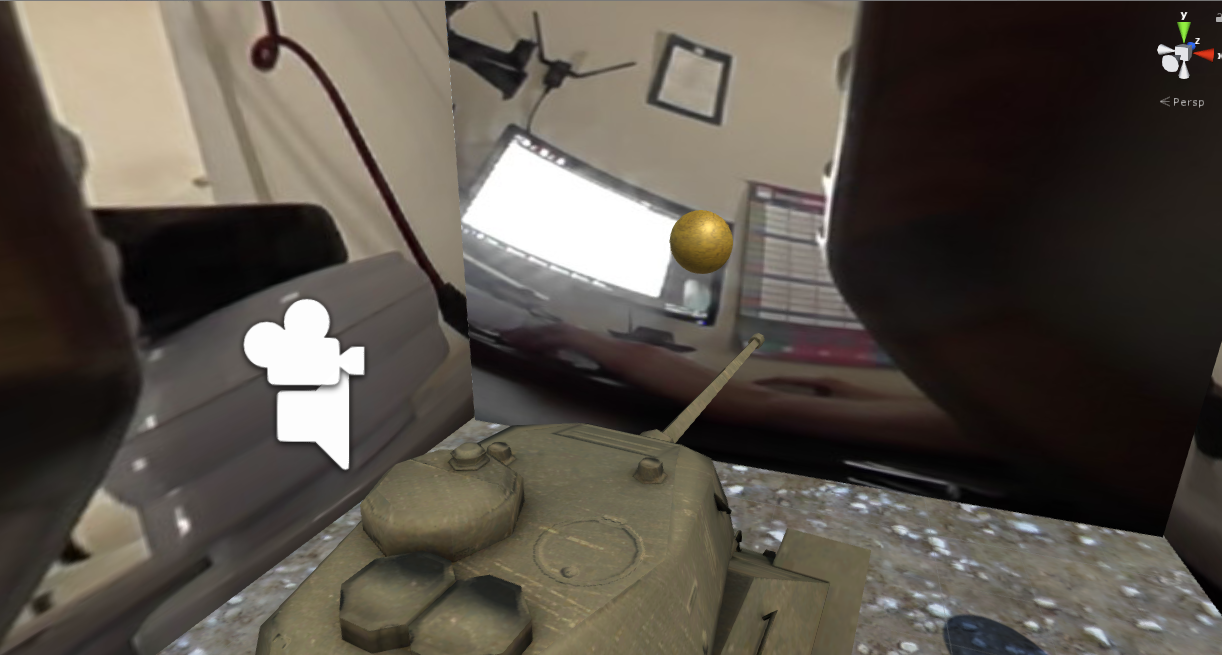
\includegraphics[width=\linewidth]{project/images/scene2.PNG}
		\caption{Old cube view}
		\label{fig:oldLook}
	\end{subfigure}	
	\begin{subfigure}[b]{0.24\textwidth}
		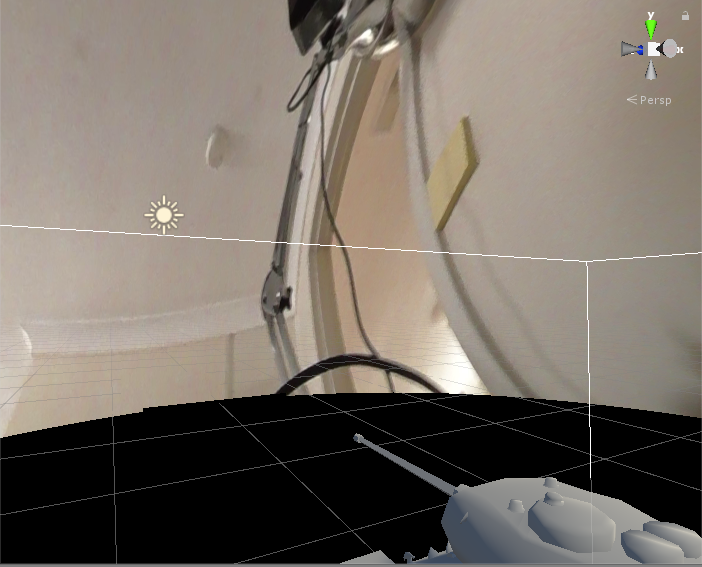
\includegraphics[width=\linewidth]{project/images/newLook1.PNG}
		\caption{New Spherical texture view}
		\label{fig:newLook}
	\end{subfigure}
	\caption{Images from Unity second usage}\label{fig:scene-developemt}
\end{figure}

\subsubsection{FFmpeg}
The most obvious approach, and the most successful one, was to modify a video stream with extra space and borders so that the relevant part of the video would appear as half of the sphere, the rest would be covered as a black area and will go beneath the Virtual view.
The Autogen version of FFmpeg inside Unity misses the following library: \textit{avformat-57}.
Directly copy/paste \textit{.dll} the file will not work out in this case.
Such operation requires recompilation of the entire build.
However, it was decided by the supervisor to use an independent build.\\
The FFmpeg with version 3.2 with the shared configuration~\cite{fate_ffmpeg_2018} build was able to capture the stream from the camera IP address \textit{(172.16.0.254:9176)} and modify with the following commands.
\begin{lstlisting}
    Input Command:
    ffmpeg -i http://172.16.0.254:9176/ -vf \
        "pad=width=2048:height=1024:x=512:y=0:color=black" \
        -vcodec mpeg4 -f mpegts udp://127.0.0.1:23001
    Siccesfull output:
        Stream #0:0: Video: mjpeg, yuvj422p(pc,bt470bg/
        unknown/unknown), 1024x1024, 25 tbr, 25 tbn, 25 tbc
\end{lstlisting}
Two boundary boxes are placed from both sides of a video stream so that they will fill the space at the bottom of the sphere. 
The following equation can describe the process of manual computing better:
\begin{align*}
    Given:\ H:1024,\ W:1024 \\
    PadSizeW&=W/2\ \&\ PadSizeH=\simeq (1-3) \\
    PadLocX1&=512 \ \&\ PadLocY1=0 \\
    PadLocX2&=W-512 \ \&\ PadLocY1=H \\
    ResultedVideoW&=W+2*(PadSizeW)=2048 \\
    ResultedVideoH&=H+2*(PadSizeH)=(1025-1034) \\
    Therefore: ResultedVideo\ H:(1025-1034),\ W:2048
\end{align*}
The address for access is presented below.
Using UDP protocol, Unity was able to capture that and produce the expected texture over the surroundings.
\begin{align*}
    udp://127.0.0.1:23001
\end{align*}
\textbf{Additional Commands which was used upon usage to concrete testing videos:}
\begin{lstlisting}
    list.txt:
        file '111_0001.MP4'
        file '111_0002.MP4'
        file '111_0003.MP4'
        file '111_0004.MP4'
    ----
    ffmpeg -safe 0 -f concat -i list.txt -c copy PreVideo.mp4
    ----
    ffmpeg.exe -i PreVideo.mp4 -vf \
        "pad=width=4320:height=2880:x=720:y=0:color=black" \
        -c copy output.mp4
\end{lstlisting}

\subsubsection{TensorFlow usage for ML}
%\textbf{Model integration into the thing. Seting up to .NET 4.6 Equivalent}
% File > Build Settings > Player Settings > Other Settings > Configuration > Scripting Runti
% Enable Tensorflow
The setup and usage of TensorFlow turned out to be much more complicated than it appeared initially.
The RTX2080Ti graphics cards have a new CUDA Compute capability level, which is not yet commonly used in primary TF libraries.  \\
\textit{Please consider a warning that if someone is planning to perform the installation, consider the following things:}
\begin{enumerate}
    \item Final build product may consume up to 15-20GB memory per compatibility support. 
The usage of RAM is very high and requires at least 6-8 GB; if this is not possible, consider the usage of flags, which will limit memory consumption.
    \item The process is very long, up to half an hour or more.\footnote{I managed to cook both lunch and dinner while the I7 overclocked processor was performing 6437 tasks in parallel with 12 threads.}
    \item Cease all activities before building.
    \item Installation process generally safe, as long as the machine is in working condition and keeps proper cooling effect\footnote{As a safety check, except for water cooling, compilation processed with three additional fans}.
\end{enumerate}
The next process will describe how the installation process went through:
\begin{multicols}{2}
\begin{enumerate}
    \item The steps for installation was taken from official Tensorflow website.\cite{tensorflow_build_2019}
    \item Python and setup environment configured with the help of Anaconda3. The separate environment used Python version 3.5. Any higher versions are not supported.        
    \item MSYS2 with the latest version had no issue in installation. It serves only as an environment for some Linux commands.
    \item GPU support required the following packages and their versions: 
    \begin{enumerate}
        \item CUDA 10.1
        \item cuDNN 7.4.2
        \item TensorRT 4.2
        \item Baze 0.19.2. WARNING! \footnote{Any younger or older version is unstable with Tensorflow. It was a matter of trials and error to get the appropriate one.} 
        \item XJN configuration is DISABLED
        \item AVX Support is ENABLED
    \end{enumerate}        
    \item Version of TF used for the build is 1.13r0
    \item Buidling Process was performed withn VS2015 x64 Native Tools CMD.
\end{enumerate}
\end{multicols}
The configuration and instructions above have to produce a proper wheel file, \".whl\" which is used to set up the Python PIP package manager. 
The command for building and installing is as follows:
\begin{lstlisting}
	Building with Bazel:
	bazel build --config=opt --define=no_tensorflow_py_deps=true
	            //tensorflow/tools/pip_package:build_pip_package
	
	Producing wl file:
	bazel-bin\tensorflow\tools\pip_package\build_pip_package
	            ../tensorflow-build/tensorflow_pkg

	Install wl file with PIP:
	pip install ..\tensorflow-build\tensorflow_pkg\
	            tensorflow-1.13.1-cp36-cp36m-win_amd64.whl
\end{lstlisting}
File path locations may vary depending on file structure. All work here is performed in the user home directory, with one folder:
\begin{lstlisting}
	C:/Users/User/Development/
\end{lstlisting}
As a result, GPU has shown incredible efficiency results in machine learning tasks. The whole procedure was worth it. \\
In the end, the small and efficient \textit{MobileNet} model was built to recognise all objects within the video stream.
The ml-agent prefab allowed to test the model and all remaining features of Unity itself.
The table with Keras benchmarks was moved to the Appendix~\ref{fig:keras}.
Benchmarks taken from Keras website~\cite{noauthor_applications_2018}.
\subsubsection{Socket communication}
Socket Communication was tested between Unity and Python within the same network.
ZMQ Library~\cite{omq_pyzmq_2019} has proven to be very useful for quick message exchange without additional configurations.
According to plans, Raspberry Pi will work as a server-side, then unity acts as a client and sends control commands in sequence. 
The server responds with results if it was successful or not, in case the tank gets stuck somewhere.
The testing was performed using TCP protocol under the following address.
\begin{equation}
    tcp://192.168.1.4:9999    
\end{equation}
Consider the usage of \textit{Nmap} tool for discovering which R-Pi has used IP address at initial connection.